\lab{One-Dimensional Optimization}{One-Dimensional Optimization}
\label{lab:1-dOpt}

\objective{
One-dimensional optimization methods find numerical approximations of the minima of functions that are unimodal on a specified domain (they only have one local minimizer on the domain). 
They do so by evaluating the function (or its derivatives) at carefully selected points on the domain.
In this lab, we will dicuss a few common one-dimensional optimization methods, each of which has varying degrees of effectiveness and speed.
We will then discuss how to use line searches to find a good step size.
One method called backtracking will later be important in multi-dimensional optimization as it can be used to find optimal scalar-valued parameters, such as step sizes. 
}

\section*{Golden Section Search} % -----------------------------------------

The \emph{golden section search} finds the minumum $x^*$ of a unimodal function $f:[a,b]\rightarrow\mathbb{R}$ by iteratively defining smaller intervals where $x^*$ must lie.
This method is especially useful when information about the function's derivative does not exist, is not known, or is costly to compute.

To find a smaller interval where $x^*$ must lie, strategically choose testing points
\begin{align*}
\tilde{a} &= b - \frac{b - a}{\phi}\\
\tilde{b} &= a + \frac{b - a}{\phi}
\end{align*}
where $\phi = \frac{1 + \sqrt{5}}{2}$ is the \emph{golden ratio} \footnote{Note that this is the same as $\tilde{a} = a + \rho(b-a)$ and $\tilde{b} = a + (1-\rho)(b-a)$ where $\rho = \frac{3-\sqrt{5}}{2}$.}.
These points are strategic as they create evenly sized intervals $[\tilde{a}, b]$ and $[a, \tilde{b}]$.
In fact, these intervals are \emph{golden sections} as the ratio of the lengths of $[a,\tilde{a}]$ and $[\tilde{a},b]$ is the same as the ratio of the lengths of $[\tilde{a}, b]$ and $[a, b]$.
Additionally, the property of the golden ratio that  $\frac{1}{\phi^2} = 1 - \frac{1}{\phi}$ leads to a smaller amout of computations needed.
Please see the Additional Material for a derivation of both of these facts.

Now consider the following three cases.
If $f(\tilde{a}) < f(\tilde{b})$, then the function cannot decrease on $[\tilde{b}, b]$ due to the fact that it increased on $[\tilde{a}, \tilde{b}]$ and is unimodal (Refer to Figure \ref{linesearch:gs}).
Thus, $x^*\in [a, \tilde{b}]$.
By similar reasoning, if $f(\tilde{a}) > f(\tilde{b})$ , then $x^* \in [\tilde{a}, b]$.
If $f(\tilde{a}) = f(\tilde{b})$, then the unimodality of $f$ does not give us any information about where the minimizer may lie.
To continue iterating, let $x^*\in [a, \tilde{b}]$ or $x^*\in[\tilde{a}, b]$ (but the method is not guaranteed to converge to the local minimum if this is the case).
Continue this iterative proccess on the smaller interval until a desired stopping criteria.
Once this criteria is reached, the minimum can be approximated as the midpoint of the final interval.
This method converges linearly.

\begin{figure}[H]
\centering
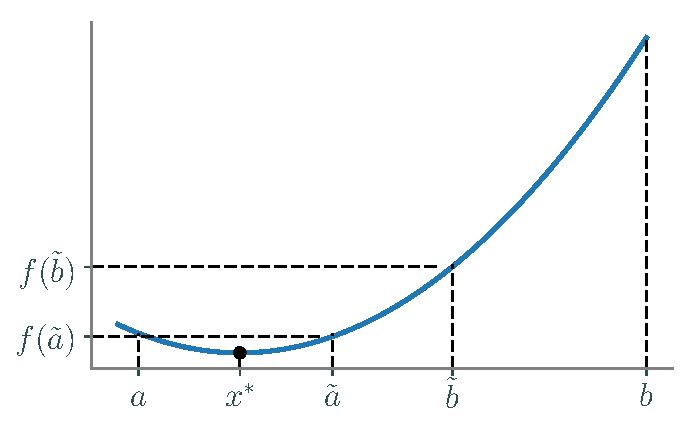
\includegraphics[width=.7\textwidth]{figures/golden_section.pdf}
\caption{An illustration of using the golden section method to optimize a unimodal function. As $f(\tilde{a}) < f(\tilde{b})$, $x^*$ must be in the interval $[a, \tilde{b}]$.}
\label{linesearch:gs}
\end{figure}

\begin{algorithm}[H]
\begin{algorithmic}[1]
\Procedure{golden\_section}{$f,\hspace{0.02in}a,\hspace{0.02in}b$,\hspace{0.02in}tol,\hspace{0.02in}maxiters}
   \State $x_0 \gets (a + b)/2$
        \Comment{Set the initial minimizer approximation.}
   \State $\phi = (1+\sqrt{5})/2$
        \Comment{Set $\phi$.}
   \For{i=0\dots maxiters}
       \Comment Update the approximation a maximum number of times.
        \State $\tilde{a} \gets b - (b - a)/\phi$
            \Comment{Set $\tilde{a}$.}
        \State $\tilde{b} \gets a + (b-a)/\phi$
            \Comment{Set $\tilde{b}$. }
        \If{$f(\tilde{a}) \leq f(\tilde{b})$}
              \Comment{Set the new boundaries of the interval}
              \State $b \gets \tilde{b}$
         \Else{}
               \State $a \gets \tilde{a}$
                \EndIf
        \State $x_1 = (a + b)/2$
             \Comment{Set the minimizer approximation.}
        \If{$|x_0-x_1| <$ tol}
              \State break
                      \Comment{Break out of the loop if the tolerance has been reached}
	   \EndIf
        \State $x_0 = x_1$
                      \Comment{Update the approximations.}
   \EndFor
   \Return $x_0$
\EndProcedure
\end{algorithmic}
\caption{The Golden Section Search}
\label{Alg:Golden-Section-Search}
\end{algorithm}

\begin{problem}
Write a function that accepts a callable function $f$, interval limits $a$ and $b$, a stopping tolerance \li{tol}, and a max number of iterations \li{maxiters}.
Implement the golden section search and return the minimizer approximation, whether or not the algorithm converged (bool), and the number of iterations executed.

Test your function by minimizing $f(x) = e^x - 4x$ on the interval $[0, 3]$, and by comparing your results to the results of \li{scipy.optimize.golden()}.
The following code shows how to use \li{scipy.optimize.golden()}.
 
\begin{lstlisting}
>>> from scipy import optimize as opt
>>> import numpy as np

>>> f = lambda x : np.exp(x) - 4*x
>>> result = opt.golden(f, brack=(0,3), tol=.001)
\end{lstlisting}
\label{prob:golden-section-search}
\end{problem}

\section*{Newton's Method} % =========================

\emph{Newton's method} is a root finding method that can be used to find optimal values.
It requires the ability to evaluate a function's first and second derivatives at specified points $(x_k)_{k=1}^n$.
For each $x_k$, it uses the points $f(x_k)$, $Df(x_k)$, and $D^2 f(x_k)$ to fit $f$ with a quadratic
$$q(x) = f(x_k) + Df(x_k) (x - x_k) + \frac{1}{2} D^2 f(x_k) (x - x_k)^2$$
found using a Taylor expansion (see Figure \ref{linesearch:quadratic}).
It then uses the critical value of $q(x)$ as the subsequent approximation $x_{k+1}$ for the minimizer as follows:
\begin{align*}
0 &= q'(x) = Df(x_k) + D^2 f(x_k)(x-x_k) \\
x_{k+1} &= x_k - \frac{Df(x_k)}{D^2 f(x_k)} \\
\end{align*}
where $x_{k+1}$ was plugged into for $x$ and solved for.

\begin{figure}[H]
\centering
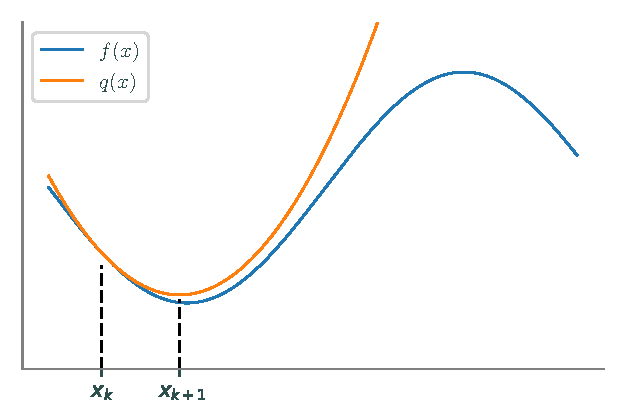
\includegraphics[width = .7 \textwidth]{figures/quad_approx.pdf}
\caption{A quadratic approximation of $f$ at $x_k$.
Note that the minimum of $q(x)$, $x_{k+1}$, is close to the minimum of $f$.
Also note that an initial starting point close to the right side of the graph could cause problems with Newton's method.
Namely, it could cause the algorithm to converge to a (non-global) local minimum.
Furthermore, the fact that $D^2 f(x) < 0$ in this domain could affect the ability of the algorithm to converge.}
\label{linesearch:quadratic}
\end{figure}

As Newton's method approximates $f$ with a quadratic, it works fairly well when $D^2 f(x) > 0$ on the entire domain; otherwise, it may fail to converge.
When it converges, it does so quadratically.
In order for it to converge to the global minimum, when $f$ is not unimodal, the initial guess $x_0$ must be sufficiently close to $x^*$.

\begin{problem}
Write a method that accepts a function $f$'s first and second derivatives as callable functions $df$ and $d2f$, a starting point $x0$, a stopping tolerance \li{tol}, and a max number of iterations \li{maxiters}.
Implement Newton's Method as described above and return the minimizer approximation, whether or not the algorithm converged (bool), and the number of iterations executed.

Test your function by minimizing $f(x) = x^2 + \sin(5x)$ with an initial guess of $x_0 = 0$, a stopping tolerance of $10^{-10}$, and $500$ max iterations.
Compare it to \li{scipy.optimize.newton()} to check your answers.
Be aware, however, that it is a root finding function, and as such will need to passed the first and second derivatives as follows:
\begin{lstlisting}
>>> df = lambda x : 2*x + 5*np.cos(5*x)
>>> d2f = lambda x : 2 - 25*np.sin(5*x)
>>> result = opt.newton(df, x0 = 0, fprime = d2f, tol = 1e-10, maxiter = 500)
# If fprime is not provided, the Secant method will be used.
\end{lstlisting}
Note that other initial guesses can yield different minima for this function.
\end{problem}

\subsection*{Secant Method} % ---------------------------------

When the second derivative of a function is not available or is computationally expensive, a \emph{Quasi-Newton method} could be used.
These methods perform Newton's method with a numerically approximated second derivative.
The \emph{Secant method} approximates it using secant lines, or in other words, the rate of change between points.
The approximation can be thought of as a difference quotient\footnote{An equation of the form $\frac{f(x + h) - f(x)}{h}.$} where $h = \Delta x$.
Thus, $$D^2 f(x_n) \approx \frac{Df(x_n) - Df(x_{n-1})}{x_n - x_{n-1}}.$$
This defines a new search method equation as follows:
$$x_{n+1} = x_n - \frac{x_n - x_{n-1}}{Df(x_n) - Df(x_{n-1})}Df(x_n).$$
This method converges superlinearly, with convergence criteria similar to Newton's method. 
Notice that this equation requires two initial points (both $x_n$ and $x_{n-1}$) to calculate the next estimate.

\begin{problem}
Write a function that accepts a first derivative $df$, starting points $x0$ and $x1$, a stopping tolerance \li{tol}, and a max number of iterations \li{maxiters}.
Implement the Secant method as described above and return the minimizer approximation, whether or not the algorithm converged (bool), and the number of iterations executed.

Test your code with the function $f(x) = x^2 + \sin(x) + \sin(10x)$ and with initial guesses of $x_0 = 0$ and $x_1 = -1$.
Compare your answer with the graph of the function.
Note that this function is highly sensitive to the starting point, which is why it is not as helpful to compare your function with SciPy's method.
As noted above, \li{scipy.optimize.newton()} uses the Secant method when the second derivative is not available.
The only difference in the syntax is that the \li{fprime} argument is not included.
This means that the function only takes in one initial condition, so it could converge to a different minimum.
\end{problem}

\section*{Descent Methods} % ========================================

\emph{Descent methods} are optimization algorithms that create successive approximations ($\textbf{x}_0$, $\textbf{x}_1$,  $\textbf{x}_2$, ...) to a minimizer by descending towards it.
They can be written in the form
\begin{equation}
\textbf{x}_{k+1} = \textbf{x}_k + \alpha_k \textbf{p}_k
\label{eq:descent}
\end{equation}
where $\alpha_k$ is the \emph{step size} and $\textbf{p}_k$ is the \emph{search direction}.

To be effective, these methods must use a good step size $\alpha_k$.
If $\alpha_k$  is too large, the method will overstep the minimum (refer to Figure \ref{fig:alpha}).
If it is too small, the method will converge slowly and become computationally expensive.
To find a good value of $\alpha_k$, one-dimensional optimization may be used.
When a one-dimensional optimization method is used to find a step size, it is referred to as a \emph{line search}.

\begin{figure}[H]
\centering
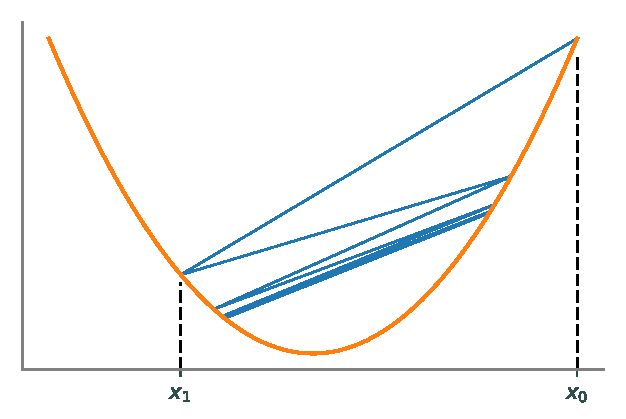
\includegraphics[width=.7\textwidth]{figures/large_alpha.pdf}
\caption{When $\alpha_k$ is too large, a descent method will overstep the minimizer. }
\label{fig:alpha}
\end{figure}

\subsection*{Step Size Calculation} % ======================================

Any one-dimensional optimization method can be used to find an optimal step size $\alpha_k$ by minimizing $\phi_k(\alpha) =  f(\textbf{x}_k + \alpha\textbf{p}_k)$.
In practice, doing this at every iteration is not always practical, as it may be too computationally expensive.
Often computational resources could be more efficiently employed finding a better search direction than a better step size.
Thus, other methods have been derived to find a step size that may not be optimal, but good enough.
These methods do not seek to minimize $\phi_k(\alpha)$, but instead seek to sufficiently decrease it.

The most common approach is to find an $\alpha_k$ that satisfies the \emph{Wolfe conditions}:
\begin{align*}
&f(\textbf{x}_k + \alpha_k \textbf{p}_k) \leq f(\textbf{x}_k) + c_1\alpha_k\nabla f(\textbf{x}_k)\trp \textbf{p}_k  \\
& -\nabla f(\textbf{x}_k + \alpha_k \textbf{p}_k)\trp \textbf{p}_k \leq -c_2\nabla f(\textbf{x}_k)\trp \textbf{p}_k
\end{align*}
where $0 < c1 < c2 < 1$ (for the  best results, choose $c1 << c2$).
The first condition is often referred to as the \emph{Armijo condition}.
It ensures that each step decreases $f$.
But this condition is not enough on its own.
By Taylors theorem,
$$f(\textbf{x}_k + \alpha_k \textbf{p}_k) = f(\textbf{x}_k) + \alpha_k\nabla f(\textbf{x}_k)\trp \textbf{p}_k + \mathcal{O}(\alpha_k^2).$$
Thus, a very small $\alpha_k$ will always satisfy the Armijo condition (note that as $\textbf{p}_k$ is a descent direction, $f(\textbf{x}_k)\trp\textbf{p}_k < 0$).
As a small step size is not always effective, the second Wolfe condition, also known as the \emph{curvature condition}, must also be satisfied.

It is possible to find an $\alpha_k$ that satisfies the Wolfe conditions, but is far from the minimizer of $\phi_k(\alpha)$.
To ensure an $\alpha_k$ is near the minimizer, the \emph{Strong Wolfe conditions} must be used.
These conditions modify the curvatuve condition, so that it is now
$$ |\nabla f(\textbf{x}_k + \alpha_k \textbf{p}_k)\trp \textbf{p}_k| \leq c_2|\nabla f(\textbf{x}_k)\trp \textbf{p}_k|.$$

Another set of conditions that can be used is called the \emph{Armijo - Goldstein conditions}
$$ f(\textbf{x}_k) + (1 - c)\alpha_k\nabla f(\textbf{x}_k)\trp \textbf{p}_k \leq f(\textbf{x}_k + \alpha_k\textbf{p}_k) \leq f(\textbf{x}_k) + c\alpha_k\nabla f(\textbf{x}_k)\trp\textbf{p}_k$$
where $0 < c < 1$.
These conditions are very similar to the Wolfe conditions (note that the right inequality is the Armijo condition). 
However, they do not require the calculation of the directional derivative $\nabla f(\textbf{x}_k + \alpha_k \textbf{p}_k)\trp\textbf{p}_k$.
They perform as well as the Wolfe conditions in most situations, but are not well-matched for quasi-Newton methods with positive definite Hessians.

\subsubsection*{Backtracking} % --------------------------------------------------

\emph{Backtracking} is a line search algorithm that can be used to find a value of $\alpha_k$ that satisfies certain conditions.
It starts with an initial step size $\alpha$, and repeatedly scales it down by a factor $\rho$ until the conditions are satisfied.
The algorithm below only requires $\alpha$ to satisfy the Armijo-condition.
This is usually sufficient, but if it finds $\alpha$'s that are too small, the algorithm can be modified to satisfy the curvature or Goldstein conditions as well.

\begin{algorithm}[H]
\begin{algorithmic}[1]
\Procedure{backtracking}{$f,\hspace{0.02in}df,\hspace{0.02in}\textbf{x},\hspace{0.02in}\textbf{p},\hspace{0.02in}\alpha,\hspace{0.02in}\rho,\hspace{0.02in}c$}
	\State $\textbf{dfp}\gets df(\textbf{x})\trp\textbf{p}$
		\Comment{Compute these values only once.}
	\State $\textbf{fx}\gets f(\textbf{x})$
	\While{$\big(f(\textbf{x}_k + \alpha\textbf{p}_k) > \textbf{fx} + c\hspace{0.01in}\alpha\hspace{0.01in}\textbf{dfp}\big)$}
		\State $\alpha \gets \rho\alpha$
	\EndWhile
	\Return $\alpha$
\EndProcedure
\end{algorithmic}
\caption{Backtracking using the Armijo Condition}
\label{Alg:backtracking}
\end{algorithm}

\begin{problem}
Write a function that accepts a callable function $f$, its gradient $df$, approximation $\textbf{x}$, search direction $\textbf{p}$, initial step length $\alpha$, and parameters $\rho$ and $c$.
Implement the backtracking algorithm using the Armijo condition and return the optimal step size.

\li{scipy.optimize.linesearch.scalar_search_armijo()} finds an optimal step size using the Armijo conditions.
It may not give the exact answer as your implementation as it decreases $\alpha$ differently, but the answers should be similar.
\begin{lstlisting}
# Recall that autograd takes the derivatives of functions.
>>> from autograd import grad

>>> f = lambda x: x[0]**2 + x[1]**2 + x[2]**2
>>> x = np.array([150., .03, 40.])
>>> p = np.array([-.5, -100., -4.5])
>>> phi = lambda alpha: f(x + alpha*p)
>>> derphi = grad(phi)
>>> alpha, _ = opt.linesearch.scalar_search_armijo(phi, phi(0.), derphi(0.))

\end{lstlisting}
\end{problem}

\section*{Additional Material}

\subsection*{Golden Search Derivations}

The ratio of the lengths of $[a, \tilde{a}]$ and $[\tilde{a}, b]$ is the same as the ratio betwen the lengths of $[\tilde{a}, b]$ and $[a, b]$ as follows:
\begin{align*}
\frac{\tilde{a}-a}{b-\tilde{a}} &= \frac{(b-a)(1-\frac{1}{\phi})}{b-b+\frac{b-a}{\phi}} \\
&= \phi(1-\frac{1}{\phi}) \\
\frac{b-\tilde{a}}{b-a} &= \frac{1}{\phi}
\end{align*}
As one of the properties of the golden ratio states that $\frac{1}{\phi^2} = 1 - \frac{1}{\phi}$, they are equal.

Chosing the test points according to the golden ratio saves on computations.
For example, consider the case where $f(\tilde{a}) > f(\tilde{b})$ and label $a_0 = a$ and $a_1 = \tilde{a}$.
Thus, $x^* \in [\tilde{a}, b]$ and for the next iteration
\begin{align*}
\tilde{a_1} &= b - \frac{b - a_1}{\phi} \\
&= b - \frac{b - b + \frac{b - a_0}{\phi}}{\phi}\\
&= b - \frac{b - a_0}{\phi^2}\\
&= a_0 + \frac{b - a_0}{\phi}\\
&= \tilde{b}
\end{align*}
Therefore, the next $\tilde{a}$ is the previous $\tilde{b}$.
Similarly, if $f(\tilde{a}) < f(\tilde{b})$, then the next $\tilde{b}$ will be the previous $\tilde{a}$.